\documentclass[UTF8,fontset=none,12pt]{ctexart}

\setCJKmainfont{Songti SC}
\setCJKsansfont{PingFang SC}
\setCJKmonofont{Songti SC}

\usepackage[a4paper,margin=2.35cm]{geometry}
\usepackage{amsmath,amssymb,amsthm,mathtools,bm}
\usepackage{graphicx}
\usepackage{float}
\usepackage{booktabs}
\usepackage{array}
\usepackage{enumitem}
\usepackage[hidelinks]{hyperref}

\title{数值线性代数\quad 第 38 讲：共轭梯度法}
\author{Lloyd N. Trefethen、David Bau III\\中文阅读版}
\date{}

\begin{document}
\maketitle

\noindent
\textbf{原书页码：}293--302；\quad
\textbf{目标 PDF 页码：}308--317。

共轭梯度（conjugate gradient，CG）迭代是“最初的”Krylov 子空间迭代，
也是这类方法中最著名、最重要的科学计算方法之一。它由 Hestenes 和 Stiefel
于 1952 年发现；当特征值分布良好时，它能够极快地求解对称正定方程组。

\section*{最小化残量的 2-范数}

和前两讲一样，设 $A\in\mathbb R^{m\times m}$ 为实对称矩阵。我们希望求解
非奇异方程组

\[
Ax=b,
\]

其精确解记为 $x_\ast=A^{-1}b$。令 $\mathcal K_n$ 表示由 $b$ 生成的第 $n$
个 Krylov 子空间：

\begin{equation}
\mathcal K_n=\operatorname{span}\{b,Ab,\ldots,A^{n-1}b\}.
\tag{38.1}
\end{equation}

一种基于这个 Krylov 子空间的方法是 GMRES。按照第 35 讲的描述，在第 $n$
步，GMRES 选择 $x_n\in\mathcal K_n$，使残量
$r_n=b-Ax_n$ 的 2-范数 $\lVert r_n\rVert_2$ 最小。

不过，通常的 GMRES 算法在最小化 $\lVert r_n\rVert_2$ 时做了超过必要的工作。
由于 $A$ 是对称的，可以使用基于三项递推而不是 $(n+1)$ 项递推的更快算法。
其中一种方法称为共轭残量法（conjugate residuals）或 MINRES（minimal
residuals，最小残量法）。这些方法如果要同时适用于正定和不定矩阵，会带来
一些额外复杂性；下面直接转向更简单、也更重要的正定情形。

\section*{最小化误差的 $A$-范数}

现在进一步假设 $A$ 不仅实对称，而且正定。正如第 23 讲所述，这意味着
$A$ 的全部特征值为正，等价地，对任意非零 $x\in\mathbb R^m$ 都有
$x^TAx>0$。在这一假设下，定义

\begin{equation}
\lVert x\rVert_A=\sqrt{x^TAx}.
\tag{38.2}
\end{equation}

它是 $\mathbb R^m$ 上的一个范数，可以直接由范数定义（3.1）验证。它称为
$A$-范数。如果 $W^TW=A$（例如 $W$ 是 $A$ 的 Cholesky 因子），那么它也就是
$\lVert Wx\rVert_2$。

我们关心的向量是第 $n$ 步的误差
$e_n=x_\ast-x_n$。共轭梯度迭代可以描述为：通过一组递推公式，生成唯一的
序列 $\{x_n\in\mathcal K_n\}$，使得每一步的 $\lVert e_n\rVert_A$ 都最小。

\section*{共轭梯度迭代}

下面给出 Hestenes 和 Stiefel 使之闻名的迭代。先不解释动机，之后先推导
正交性，再把这些性质转化为最优性结论；最后从非线性优化的角度解释动机。

\begin{center}
\fbox{\begin{minipage}{0.90\textwidth}
\textbf{算法 38.1\quad 共轭梯度（CG）迭代}

\[
x_0=0,\qquad r_0\leftarrow b,\qquad p_0=r_0.
\]

\begin{align*}
\text{对 }n=1,2,3,\ldots:\qquad
\alpha_n&=\frac{r_{n-1}^Tr_{n-1}}{p_{n-1}^TAp_{n-1}}
&&\text{步长},\\
x_n&=x_{n-1}+\alpha_np_{n-1}
&&\text{近似解},\\
r_n&=r_{n-1}-\alpha_nAp_{n-1}
&&\text{残量},\\
\beta_n&=\frac{r_n^Tr_n}{r_{n-1}^Tr_{n-1}}
&&\text{本步的改进系数},\\
p_n&=r_n+\beta_np_{n-1}
&&\text{搜索方向}.
\end{align*}
\end{minipage}}
\end{center}

在分析这些公式的数学性质之前，先看它们在计算上的含义。CG 迭代非常简单，
用几行 MATLAB 就可以编程实现。它只处理 $m$-维向量，而不需要逐个处理矩阵
或向量条目，因此甚至比带选主元的高斯消去还简单。唯一没有在这里讨论的
实际问题，是如何选择收敛判据。

每一步 CG 迭代包含若干向量运算和一次矩阵--向量乘法；算法列表中
$Ap_{n-1}$ 出现两次，但只需计算一次。如果 $A$ 稠密且没有结构，这次
矩阵--向量乘法占主导地位，每步约需 $2m^2$ 次浮点运算。如果 $A$ 稀疏，
或存在其他可利用的结构，使得 $Ap_{n-1}$ 只需 $O(m)$ 次运算，那么每步的
运算量也可以低至 $O(m)$。

从算法的五行公式可以推出下面的性质。和本书中没有明确提及舍入误差的定理
一样，下面的定理假定精确算术。存在舍入误差时，这些性质会失效，而 CG
仍然能保持惊人性能的原因也会变成一个微妙问题。

\textbf{定理 38.1.}
将算法 38.1 应用于对称正定问题 $Ax=b$。只要迭代尚未收敛（即
$r_{n-1}\ne0$），算法就不会发生除以零，并且有以下子空间恒等式：

\begin{equation}
\begin{aligned}
\mathcal K_n
&=\operatorname{span}\{x_1,x_2,\ldots,x_n\}\\
&=\operatorname{span}\{p_0,p_1,\ldots,p_{n-1}\}\\
&=\operatorname{span}\{r_0,r_1,\ldots,r_{n-1}\}\\
&=\operatorname{span}\{b,Ab,\ldots,A^{n-1}b\}.
\end{aligned}
\tag{38.3}
\end{equation}

此外，残量彼此正交：

\begin{equation}
r_n^Tr_j=0\qquad(j<n),
\tag{38.4}
\end{equation}

搜索方向是“$A$-共轭”的：

\begin{equation}
p_n^TAp_j=0\qquad(j<n).
\tag{38.5}
\end{equation}

\textbf{证明。}
证明按 $n$ 归纳；这里给出非正式的提纲。由初始猜测 $x_0=0$ 以及
$x_n=x_{n-1}+\alpha_np_{n-1}$，归纳可知 $x_n$ 属于
$\operatorname{span}\{p_0,\ldots,p_{n-1}\}$。由
$p_n=r_n+\beta_np_{n-1}$，这个空间也等于
$\operatorname{span}\{r_0,\ldots,r_{n-1}\}$。最后，由
$r_n=r_{n-1}-\alpha_nAp_{n-1}$，它又等于
$\operatorname{span}\{b,Ab,\ldots,A^{n-1}b\}$，于是得到式（38.3）。

为了证明式（38.4），使用
$r_n=r_{n-1}-\alpha_nAp_{n-1}$ 以及
$(Ap_{n-1})^T=p_{n-1}^TA$，得到

\[
r_n^Tr_j=r_{n-1}^Tr_j-\alpha_np_{n-1}^TAr_j.
\]

若 $j<n-1$，右侧两项都由归纳假设为零。若 $j=n-1$，只要取

\[
\alpha_n=
\frac{r_{n-1}^Tr_{n-1}}{p_{n-1}^TAr_{n-1}},
\]

右侧差值就为零。这与算法 38.1 中
$\alpha_n=(r_{n-1}^Tr_{n-1})/(p_{n-1}^TAp_{n-1})$ 相同，只是把分母
$p_{n-1}^TAp_{n-1}$ 换成了 $p_{n-1}^TAr_{n-1}$。由于 $p_{n-1}$ 与
$r_{n-1}$ 相差一个属于 $\mathcal K_{n-2}$ 的向量，这一替换对分母的改变
是 $\beta_{n-1}p_{n-1}^TAp_{n-2}$，由归纳假设为零。

为了证明式（38.5），使用 $p_n=r_n+\beta_np_{n-1}$，得到

\[
p_n^TAp_j=r_n^TAp_j+\beta_np_{n-1}^TAp_j.
\]

若 $j<n-1$，归纳可知右侧两项再次都为零（此时式（38.4）已经对第 $n$
步成立）。若 $j=n-1$，只要

\[
\beta_n=-\frac{r_n^TAp_{n-1}}{p_{n-1}^TAp_{n-1}}
\]

即可使右侧和为零。利用 $r_n=r_{n-1}-\alpha_nAp_{n-1}$，这等价于

\[
\beta_n=
\frac{-\alpha_nr_{n-1}^TAp_{n-1}}
{\alpha_np_{n-1}^TAp_{n-1}}.
\]

这与算法 38.1 中
$\beta_n=(r_n^Tr_n)/(r_{n-1}^Tr_{n-1})$ 相同，只是把分子
$r_n^Tr_n$ 换成 $r_n^T(-\alpha_nAp_{n-1})$，把分母
$r_{n-1}^Tr_{n-1}$ 换成 $p_{n-1}^T(\alpha_nAp_{n-1})$。结合归纳假设
以及算法 38.1 的第 3、5 行，可以直接验证这些替换不改变结果。证毕。

\section*{CG 的最优性}

推导式（38.4）和（38.5）时，真正困难的工作已经完成。现在只需确认 CG
在每一步确实最小化 $\lVert e\rVert_A$。

\textbf{定理 38.2.}
将 CG 迭代应用于对称正定问题 $Ax=b$。如果迭代尚未收敛（即
$r_{n-1}\ne0$），那么 $x_n$ 是 $\mathcal K_n$ 中使 $\lVert e_n\rVert_A$
最小的唯一点。收敛是单调的：

\begin{equation}
\lVert e_n\rVert_A\leq\lVert e_{n-1}\rVert_A,
\tag{38.6}
\end{equation}

并且对某个 $n\leq m$ 有 $e_n=0$。

\textbf{证明。}
由定理 38.1，$x_n\in\mathcal K_n$。为了证明它是 $\mathcal K_n$ 中唯一的
最小点，任取

\[
\widetilde x=x_n-\Delta x\in\mathcal K_n,
\qquad
e=x_\ast-\widetilde x=e_n+\Delta x.
\]

于是

\[
\begin{aligned}
\lVert e\rVert_A^2
&=(e_n+\Delta x)^TA(e_n+\Delta x)\\
&=e_n^TAe_n+(\Delta x)^TA(\Delta x)+2e_n^TA(\Delta x).
\end{aligned}
\]

最后一项是 $2r_n^T(\Delta x)$，即 $r_n$ 与 $\mathcal K_n$ 中向量的内积；
根据定理 38.1，它为零。因此

\[
\lVert e\rVert_A^2=e_n^TAe_n+(\Delta x)^TA(\Delta x).
\]

只有第二项依赖于 $\Delta x$。又由于 $A$ 正定，这一项非负，且当且仅当
$\Delta x=0$ 时取到 0，即 $\widetilde x=x_n$。所以 $\lVert e\rVert_A$
在且仅在 $\widetilde x=x_n$ 时达到最小值。

定理剩余的结论也随之得到。式（38.6）的单调性来自
$\mathcal K_n\subseteq\mathcal K_{n+1}$；只要尚未收敛，$\mathcal K_n$ 是
$\mathbb R^m$ 中维数为 $n$ 的子空间，因此至多 $m$ 步必然收敛。证毕。

在浮点算术中，“至多 $m$ 步收敛”的保证是空的。对任意实机上的矩阵 $A$，
即使 $n=m$，也不一定观察到 $\lVert e_n\rVert_A$ 有决定性的下降。不过，
实践中使用 CG 的对象不是任意矩阵，而是谱性质足够良好的矩阵；这可能得益于
预处理，使得在 $n\ll m$ 时就达到所需精度（见第 32 讲）。因此，$n=m$ 时
的理论精确收敛与科学计算中实际使用 CG 的目的并不直接相关。

\section*{把 CG 看成优化算法}

我们刚才证明了 CG 的一个最优性：第 $n$ 步在所有 $x\in\mathcal K_n$ 中
最小化 $\lVert e_n\rVert_A$。事实上，从“步长”和“搜索方向”这些术语
就可以看出，它可以解释为在 $\mathbb R^m$ 上最小化一个非线性函数的标准
迭代算法。迭代的核心公式是

\[
x_n=x_{n-1}+\alpha_np_{n-1}.
\]

这正是优化中的熟悉形式：沿搜索方向 $p_{n-1}$ 移动步长 $\alpha_n$，把
当前近似 $x_{n-1}$ 更新为 $x_n$。连续执行这样的步骤，就试图找到某个
非线性函数的最小点。

是哪一个函数？按照定理 38.2，答案似乎应当是 $\lVert e\rVert_A$，或等价地
$\lVert e\rVert_A^2$。然而，虽然 $\lVert e\rVert_A^2$ 确实是 $x$ 的函数，
如果不知道精确解 $x_\ast$，就无法计算它。把 CG 解释成优化一个无法计算
的函数，显然不够“标准”。

另一方面，给定 $A$、$b$ 和 $x\in\mathbb R^m$，下列量是可以直接计算的：

\begin{equation}
\varphi(x)=\frac12x^TAx-x^Tb.
\tag{38.7}
\end{equation}

直接计算可得

\[
\begin{aligned}
\lVert e_n\rVert_A^2
&=e_n^TAe_n=(x_\ast-x_n)^TA(x_\ast-x_n)\\
&=x_\ast^TAx_\ast-2x_n^TAx_\ast+x_n^TAx_n\\
&=x_\ast^TAx_\ast-2x_n^Tb+x_n^TAx_n\\
&=2\varphi(x_n)+\text{常数}.
\end{aligned}
\]

所以 $\varphi(x)$ 与 $\lVert e\rVert_A^2$ 只相差因子 2 和未知常数
$x_\ast^Tb$。和 $\lVert e\rVert_A$ 一样，它的唯一最小点也是 $x=x_\ast$。

因此，CG 可以解释为在 $\mathbb R^m$ 上最小化二次函数 $\varphi(x)$ 的迭代
过程。每一步计算
$x_n=x_{n-1}+\alpha_np_{n-1}$，使 $\varphi(x)$ 在一维空间
$x_{n-1}+\operatorname{span}\{p_{n-1}\}$ 上达到最小。（容易验证，算法中的
$\alpha_n=(r_{n-1}^Tr_{n-1})/(p_{n-1}^TAp_{n-1})$ 在所有步长中使
$\varphi$ 最小。）CG 的特别之处在于搜索方向 $p_{n-1}$：在该方向上最小化
$\varphi$，实际上就等价于在整个 $\mathcal K_n$ 上最小化它。

CG 求解 $Ax=b$ 与 Lanczos 迭代求特征值之间存在紧密类比。第 27 讲指出，
$A$ 的特征值是 $\mathbb R^m$ 上 Rayleigh 商

\[
r(x)=\frac{x^TAx}{x^Tx}
\]

的驻值。习题 36.1 指出，Lanczos 第 $n$ 步的特征值估计（Ritz 值）正是把
$x$ 限制在 Krylov 子空间 $\mathcal K_n$ 后，这个函数的驻值。这与我们刚刚
证明的结论完全平行：$Ax=b$ 的解 $x_\ast$ 是 $\mathbb R^m$ 上标量函数
$\varphi(x)$ 的最小点，而 CG 迭代 $x_n$ 是把 $x$ 限制在 $\mathcal K_n$
后同一函数的最小点。

\section*{CG 与多项式逼近}

前四讲反复出现的主题，是 Krylov 子空间迭代与矩阵多项式之间的联系。
Arnoldi 和 Lanczos 迭代解决 Arnoldi/Lanczos 逼近问题（34.3），GMRES
解决 GMRES 逼近问题（35.10）。对 CG 来说，相应的逼近问题涉及误差的
$A$-范数：

\begin{center}
\fbox{\begin{minipage}{0.88\textwidth}
\textbf{CG 逼近问题。}
寻找 $p_n\in\mathcal P_n$，使得
\[
\lVert p_n(A)e_0\rVert_A=\min.
\tag{38.8}
\]
\end{minipage}}
\end{center}

这里 $e_0$ 是初始误差，即 $e_0=x_\ast-x_0=x_\ast$；$\mathcal P_n$ 与式
（35.7）中的定义相同，是满足 $p(0)=1$ 且次数不超过 $n$ 的多项式集合。
由定理 38.2 可以得到下面的收敛定理。

\textbf{定理 38.3.}
如果 CG 在第 $n$ 步之前尚未收敛（即 $r_{n-1}\ne0$），那么式（38.8）
有唯一解 $p_n\in\mathcal P_n$，并且第 $n$ 步误差为
$e_n=p_n(A)e_0$。因此

\begin{equation}
\frac{\lVert e_n\rVert_A}{\lVert e_0\rVert_A}
=\inf_{p\in\mathcal P_n}
\frac{\lVert p(A)e_0\rVert_A}{\lVert e_0\rVert_A}
\leq
\inf_{p\in\mathcal P_n}\max_{\lambda\in\Lambda(A)}|p(\lambda)|,
\tag{38.9}
\end{equation}

其中 $\Lambda(A)$ 表示 $A$ 的谱。

\textbf{证明。}
由定理 38.1，存在某个 $p\in\mathcal P_n$ 使
$e_n=p(A)e_0$。式（38.9）中的等号由此事实和定理 38.2 得到。对于不等号，
设 $e_0=\sum_{j=1}^m a_jv_j$，其中 $v_j$ 是 $A$ 的一组正交归一特征向量，
对应特征值 $\lambda_j$。则

\[
p(A)e_0=\sum_{j=1}^m a_jp(\lambda_j)v_j,
\]

从而

\[
\lVert e_0\rVert_A^2=\sum_{j=1}^m a_j^2\lambda_j,\qquad
\lVert p(A)e_0\rVert_A^2
=\sum_{j=1}^m a_j^2\lambda_jp(\lambda_j)^2.
\]

因此

\[
\frac{\lVert p(A)e_0\rVert_A^2}{\lVert e_0\rVert_A^2}
\leq\max_{\lambda\in\Lambda(A)}|p(\lambda)|^2,
\]

这就推出了式（38.9）中的不等式。证毕。

\section*{收敛速率}

定理 38.3 表明，CG 的收敛速率由 $A$ 的谱位置决定。所谓“好”的谱，是指
存在 $p_n\in\mathcal P_n$，使其在谱上很小，并且随 $n$ 增大而快速变小。
粗略地说，这可能来自两个原因之一，或者二者兼有：特征值聚集成小簇，
或者它们整体上与原点保持良好的相对分离。定理 38.3 的两个最著名推论
分别讨论这两种情形的极端版本。

先假设特征值完全聚集，但不对这些簇的位置作任何假设。

\textbf{定理 38.4.}
如果 $A$ 只有 $n$ 个不同的特征值，那么 CG 至多经过 $n$ 步就收敛。

\textbf{证明。}
这是式（38.9）的直接推论：存在

\[
p(x)=\prod_{j=1}^{n}\left(1-\frac{x}{\lambda_j}\right)\in\mathcal P_n,
\]

它在指定的 $n$ 个点 $\{\lambda_j\}$ 上全为零。证毕。

在另一种极端情形下，假设我们对特征值是否聚集一无所知，只知道它们到原点
的距离最多相差一个因子 $\kappa>1$。换言之，只知道 $A$ 的 2-范数条件数

\[
\kappa=\frac{\lambda_{\max}}{\lambda_{\min}},
\]

其中 $\lambda_{\max}$、$\lambda_{\min}$ 是 $A$ 的最大和最小特征值。

\textbf{定理 38.5.}
设 CG 应用于对称正定问题 $Ax=b$，且 $A$ 的 2-范数条件数为 $\kappa$。
则误差的 $A$-范数满足

\begin{equation}
\frac{\lVert e_n\rVert_A}{\lVert e_0\rVert_A}
\leq
2\left[
\left(\frac{\sqrt\kappa+1}{\sqrt\kappa-1}\right)^n+
\left(\frac{\sqrt\kappa+1}{\sqrt\kappa-1}\right)^{-n}
\right]^{-1}
\leq
2\left(\frac{\sqrt\kappa-1}{\sqrt\kappa+1}\right)^n.
\tag{38.10}
\end{equation}

\textbf{证明。}
根据定理 38.3，只需寻找一个 $p\in\mathcal P_n$，使它在
$[\lambda_{\min},\lambda_{\max}]$ 上的最大值达到式（38.10）中间的表达式。
取缩放平移后的 Chebyshev 多项式

\[
p(x)=
\frac{T_n\!\left(\gamma-\dfrac{2x}{\lambda_{\max}-\lambda_{\min}}\right)}
{T_n(\gamma)},
\qquad
\gamma=\frac{\lambda_{\max}+\lambda_{\min}}
{\lambda_{\max}-\lambda_{\min}}
=\frac{\kappa+1}{\kappa-1}.
\]

当 $x\in[\lambda_{\min},\lambda_{\max}]$ 时，$p(x)$ 分子中的
Chebyshev 多项式自变量位于 $[-1,1]$，所以分子绝对值不超过 1。因此只需证明

\begin{equation}
T_n(\gamma)
=T_n\!\left(\frac{\kappa+1}{\kappa-1}\right)
=\frac12\left[
\left(\frac{\sqrt\kappa+1}{\sqrt\kappa-1}\right)^n+
\left(\frac{\sqrt\kappa+1}{\sqrt\kappa-1}\right)^{-n}
\right].
\tag{38.11}
\end{equation}

令

\[
x=\frac12(z+z^{-1}),\qquad
T_n(x)=\frac12(z^n+z^{-n}),
\]

这是 Chebyshev 多项式的标准表示。若
$\frac{\kappa+1}{\kappa-1}=\frac12(z+z^{-1})$，则 $z$ 满足二次方程

\[
\frac12z^2-\frac{\kappa+1}{\kappa-1}z+\frac12=0.
\]

取大于 1 的根，有

\[
\begin{aligned}
z
&=\frac{\kappa+1}{\kappa-1}
+\sqrt{\left(\frac{\kappa+1}{\kappa-1}\right)^2-1}\\
&=\frac{\kappa+1+\sqrt{(\kappa+1)^2-(\kappa-1)^2}}{\kappa-1}\\
&=\frac{\kappa+1+\sqrt{4\kappa}}{\kappa-1}
=\frac{\sqrt\kappa+1}{\sqrt\kappa-1}.
\end{aligned}
\]

于是 $T_n(\gamma)=\frac12(z^n+z^{-n})$，即式（38.11）。证毕。

定理 38.5 是关于 CG 收敛的最著名结果。由于

\[
\frac{\sqrt\kappa-1}{\sqrt\kappa+1}
\sim1-\frac{2}{\sqrt\kappa}
\qquad(\kappa\to\infty),
\]

它表明：当 $\kappa$ 较大但还没有大到不可接受时，达到给定容差通常只需
$O(\sqrt\kappa)$ 次迭代。不过这只是上界；对特殊右端项（不太常见）或聚集
谱（更常见），收敛可能更快。

\section*{例}

考虑如下构造的 $500\times500$ 稀疏矩阵 $A$，作为 CG 收敛的例子。先在
每个对角位置放置 1，在每个非对角位置放置一个服从 $[-1,1]$ 均匀分布的
随机数，并保持对称性 $A=A^T$。然后对每个满足
$|a_{ij}|>\tau$ 的非对角元素，将其替换为 0，其中 $\tau$ 是参数。
当 $\tau$ 接近 0 时，所得矩阵是条件良好的正定矩阵，非零元密度约为 $\tau$。
随着 $\tau$ 增大，条件数和非零结构都会恶化。

\begin{figure}[H]
\centering
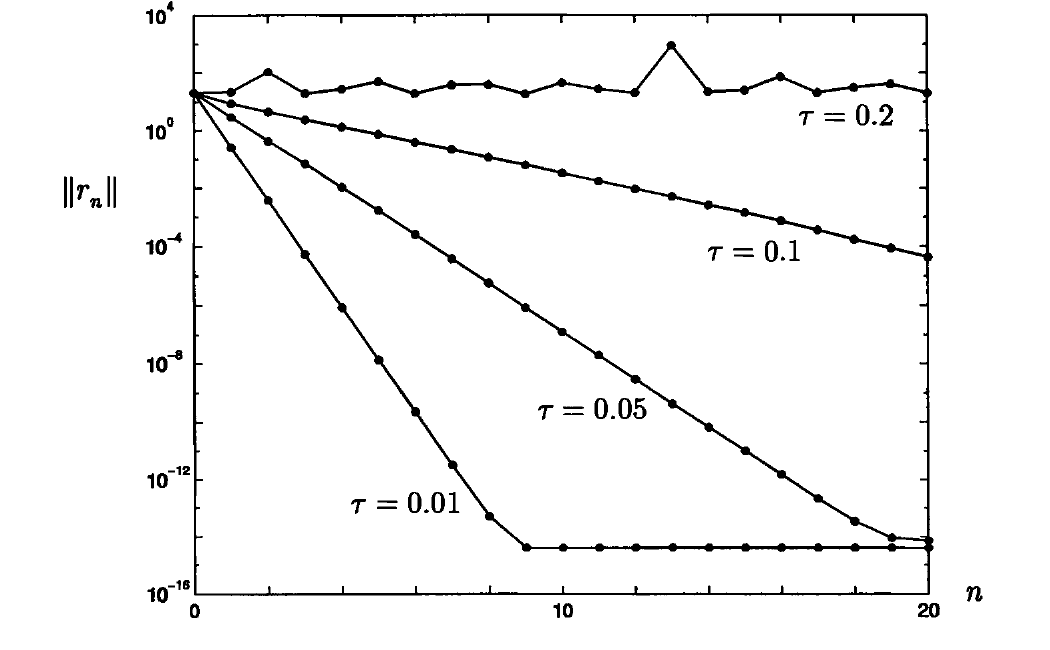
\includegraphics[width=0.92\textwidth]{../assets/figure-38-cg-convergence.png}
\parbox{0.94\textwidth}{\small 图 38.1. 文中所述 $500\times500$ 稀疏矩阵的 CG 收敛曲线。$\tau=0.01$ 时，CG 比 Cholesky 分解快约 700 倍；$\tau=0.2$ 时，矩阵不是正定的，因此没有收敛。}
\end{figure}

图 38.1 给出了这类矩阵在 CG 迭代前 20 步中的收敛曲线；右端项 $b$ 取为
随机向量。各参数的数值表现如下：

\begin{itemize}[leftmargin=2.6em]
\item $\tau=0.01$：$A$ 有 3092 个非零元，$\kappa\approx1.06$；9 步达到机器精度，
约需 $6\times10^4$ 次浮点运算。
\item $\tau=0.05$：有 13062 个非零元，$\kappa\approx1.83$；19 步收敛，
约需 $5\times10^5$ 次浮点运算。
\item $\tau=0.1$：有 25526 个非零元，$\kappa\approx10.3$；20 步后只有
约 5 位数字收敛，约需 $10^6$ 次浮点运算。
\item $\tau=0.2$：有 50834 个非零元，完全没有收敛。此时最低特征值为负，
$A$ 不再正定，使用 CG 不合适。（CG 有时也能在不定矩阵上成功，但这里的
矩阵不仅不定，而且病态。）
\end{itemize}

注意，$\tau=0.01$ 的曲线与图 32.1 的理想示意图非常接近。在这个例子中，
$6\times10^4$ 次浮点运算比 Cholesky 分解（式（23.4））快约 700 倍。
遗憾的是，即使尽力寻找良好的预条件器，实际问题中的矩阵也不一定拥有这样
规整的谱。

\section*{习题}

\paragraph{38.1.}
根据正文报告的条件数 $\kappa$，确定定理 38.5 对图 38.1 中
$\tau=0.01,0.05,0.1$ 三个矩阵所预测的收敛速率。在图 38.1 的副本上画出
相应直线，说明这些预测与实际收敛速率有多接近。

\paragraph{38.2.}
设 $A$ 是一个实对称 $805\times805$ 矩阵，其特征值为
$1.00,1.01,1.02,\ldots,8.98,8.99,9.00$，此外还有 $10,12,16,24$。
为了确保把初始误差 $\lVert e_0\rVert_A$ 降低 $10^6$ 倍，需要进行多少步
共轭梯度迭代？

\paragraph{38.3.}
CG 应用于对称正定矩阵 $A$，得到
$\lVert e_0\rVert_A=1$、$\lVert e_1\rVert_A=2\times10^{-16}$。仅根据这些
数据：

\begin{enumerate}[label=(\alph*)]
\item 能对 $\kappa(A)$ 给出什么上界？
\item 能对 $\lVert e_{20}\rVert_A$ 给出什么上界？
\end{enumerate}

\paragraph{38.4.}
设 $A$ 是稠密的对称正定 $1000\times1000$ 矩阵，且
$\kappa(A)=100$。粗略估计为了以十位数字的精度求解 $Ax=b$，以下方法
分别需要多少次浮点运算：(a) Cholesky 分解；(b) 使用最优参数 $\alpha$ 的
Richardson 迭代（习题 35.3）；(c) CG。

\paragraph{38.5.}
我们把 CG 描述成对式（38.7）的函数 $\varphi(x)$ 做迭代最小化。另一种
最小化同一函数的方法是通常更慢的最速下降法。

\begin{enumerate}[label=(\alph*)]
\item 推导 $\nabla\varphi(x)=Ax-b=-r$。因此，最速下降迭代相当于在算法
38.1 中取 $p_n=r_n$，而不是 $p_n=r_n+\beta_np_{n-1}$。
\item 确定最速下降迭代的最优步长 $\alpha_n$ 公式。
\item 写出完整的最速下降迭代。主循环内共有三个操作。
\end{enumerate}

\paragraph{38.6.}
设 $A$ 是一个 $100\times100$ 的对称三对角矩阵，对角元为
$1,2,\ldots,100$，次对角线和超对角线上的元素为 1，并令
$b=(1,1,\ldots,1)^T$。编写程序，分别进行 100 步 CG 迭代和最速下降迭代，
近似求解 $Ax=b$。绘制四条曲线：

\begin{enumerate}[label=(\alph*)]
\item CG 的计算残量范数 $\lVert r_n\rVert_2$；
\item CG 的实际残量范数 $\lVert b-Ax_n\rVert_2$；
\item 最速下降法的残量范数 $\lVert r_n\rVert_2$；
\item 定理 38.5 的估计
\[
2\left(\frac{\sqrt\kappa-1}{\sqrt\kappa+1}\right)^n.
\]
\end{enumerate}

评论你的结果。

\end{document}
